%
%
%
\section{Correlation}%
  \index{Correlation}%
  \label{sec:correlation}

Correlation is the most straightforward way to visualize, measure and estimate linear dependence between two continuous variables, by looking for a pattern in their \emph{covariance}. Stata lets you build \emph{correlation matrixes}, from which you can read \emph{correlation coefficients} for any number of variables. Correlations can be partial or `semi-partial' and can be computed onto different subsamples, depending on the exact requirements of your analysis.%

Visual inspection of your data is almost always your first step to any serious analysis, and correlation is no exception. Your starting point will be scatterplots with tentative linear fits. What you will be looking for are visual associations between pairs of variables for which there are theoretical grounds to consider that they might be \emph{correlates}.%

You will then build a correlation matrix in order to detect multiple linear codependence, which is also called \emph{multicollinearity}, among your continuous variables. Multicollinearity might require that you amend your selection of model variables, in accordance with your theoretical intuitions and research design. This process is iterative, and implies that you move back and forth between your data and your research hypotheses.%

% linear dependence, Pearson correlation

	%
	% 5.1.1
	%
  \subsection{Visualizing correlates}%
    \index{Correlation!Visualizing correlates}

  \begin{figure}
    \begin{center}
      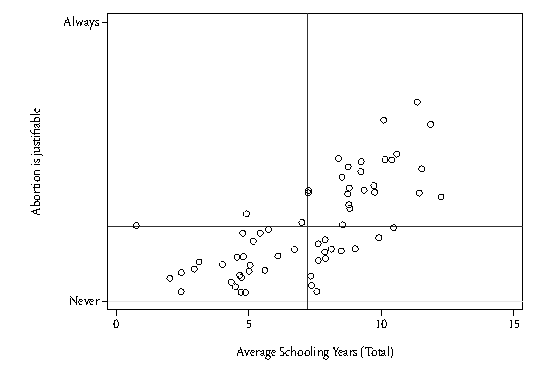
\includegraphics[width=0.48\textwidth]{images/abortion_sc_means.pdf}
    \end{center}
    	\caption[Linear correlation]{\label{fig:correlation_scatterplot}%
  	Scatterplot of support for abortion and mass education. %
    \qog}
  \end{figure}%

  Figure~\ref{fig:correlation_scatterplot} provides an example of a visual relationship to which linear regression might apply, between public opinion support for abortion and average schooling years at the population level. The visual relationship that you might detect in the data is typical of a linear \emph{correlation}. The average values of each variable are displayed on the graph to show how the data distribute around them: mostly in the bottom-left and top-right quadrants, which define a \emph{positive} linear correlation.%

  The relationships that your model will capture will be \emph{linear} ones. If you detect a quadratic or exponential relationship, correlation and regression will fail to reflect them adequately. Variable transformations can be used to circumvent this issue, but some curvilinear phenomena might persist in the data, in which case you should acknowledge this limitation in your reports.\footnote{Section~[9] covers usual variable transformations, available through the \cmd{ladder} and \cmd{gladder} commands in Stata. Ideally, your data might also justify selecting a non-linear model, as in the case of a log-linear relationship.}% \ref{sec:transformations}	

  Figure~\ref{fig:correlation_variance} offers a more detailed visualization of the variance in each variable. Recall the formulae from Section~[9] for the variance $\sigma^2$ and standard deviation $\sigma$ of a variable $X$: % ~\ref{sec:dispersion}

  $$\sigma^2_X = \text{Var}[X] = \frac{\sum (X_i - \bar X)^2}{N} \quad \text{and} \quad \sigma_X = \text{SD}_X = \sqrt{Var[X]} = \frac{\sum (X_i - \bar X)}{\sqrt{N}}$$%

  The calculation of variance involves squaring the sum of deviations between each value $X_i$ and the mean value of the distribution $\bar X$, which is then divided by the total number of observations $N$. The squared term serves to cancel out the fact that some of these deviations are positive ($X_i - \bar X > 0$), while others are negative ($X_i - \bar X < 0$).%

  Take a quick look at how support for abortion and mass education vary around their mean values in the sample:

  \begin{figure}[htp]
  	\centering
  	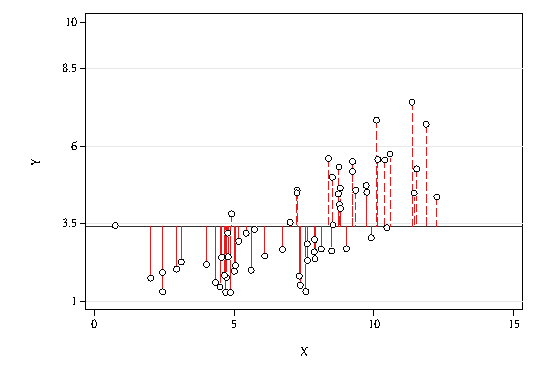
\includegraphics[width=.48\textwidth]{images/abortion_sc_yvariance.pdf}
  	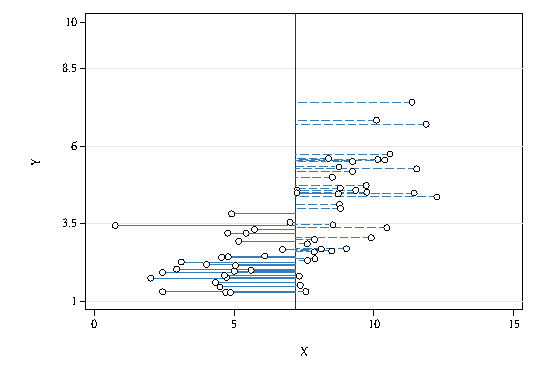
\includegraphics[width=.48\textwidth]{images/abortion_sc_xvariance.pdf}

  	\caption[Variance in two variables]{\label{fig:correlation_variance}%
  	Scatterplots of support for abortion and mass education. %
    Negative variance in solid lines, positive variance in dashed lines. %
    \qog}
  \end{figure}%

  What the graphs show at that stage is a clear association in the deviations from the mean: for the values of mass education that are \emph{above} its average level, the level of support for abortion is also \emph{above} its average level, and reversely, at levels of mass education that are \emph{below} its sample mean, support for abortion also tends to fall \emph{below} its sample mean.%

  This association is grounded in the joint variance of the two variables and can be measured as their correlation coefficient. Identically, regression relies on the joint variance of the variables included in the model to estimate its own coefficients. Both require, however, some preliminary graphical check to confirm that their relationship is effectively linear.%

Figure~\ref{fig:grmat} shows another form of correlation matrix, obtained from the \cmd{gr mat}{graph matrix} (\texttt{graph matrix}) that uses scatterplots to show every possible correlation between the variables. The matrix takes a bit of time to display, but is indispensable in any serious analysis of covariance and detection of linear relationships between \emph{all} variables included in your model. 

\begin{figure}[htp]
	\centering
	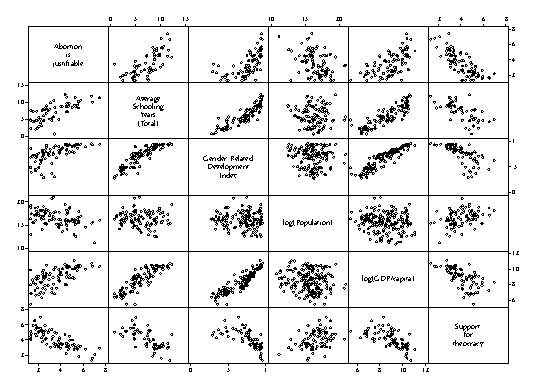
\includegraphics[width=.9\textwidth]{images/abortion_grmat.pdf}

	\caption[Scatterplot matrix with \cmd{gr mat}]{\label{fig:grmat}
	Scatterplot matrix produced with \texttt{gr mat}. \qog}
\end{figure}%

The scatterplot matrix is susceptible to confirm that several independent variables are moderately or strongly correlated, which creates \emph{interactions} within your model. The linear relationships that occur in parallel to your model create an issue called \emph{multicollinearity}, especially if you fall for the common flaw of including tons of independent variables and end up with a `kitchen-sink' model.\cite{Schrodt:2011a} Section~\ref{sec:interactions} covers this issue in detail.

At that stage, you should have obtained enough information from correlation analysis to select variables and draft your model. Correlation measures are only bivariate measures of association and can be unreliable, especially on a low number of observations: Pearson's $\rho$, for instance, requires normally distributed data to stay efficient when $N$ falls below approximately 30 observations. However, correlation is appropriate for exploratory purposes, to refine your intuitions and hypotheses before you start estimating regression models.

	%
	% 5.1.2
	%
  \index{Correlation!Coefficients}\index{Pearson's $\rho$|{Correlation}}%
  \subsection{Correlation coefficients: Pearson's $\rho$}

  Correlation is a proxy for the statistical property of \emph{linear dependence} between two variables $X$ and $Y$, which we assume when we model $Y$ as a function of $X$.\footnote{Mathematically speaking, correlation is only a proxy for linear dependence because the two notions are not strictly equivalent: two variables $X$ and $Y$ can be uncorrelated without being independent (as is actually common). Similarly, $Y$ could be expressed as a function of $X$ even if the two variables are uncorrelated, but this function would systematically fail to predict any of the variance in $Y$ from the variance in $X$. Feel free to have a drink.} Correlation can be expressed as a single coefficient $\rho (X,Y)$ that varies from perfect negative correlation when $\rho = -1$ to perfect positive correlation when $\rho = +1$. A correlation coefficient of $\rho = 0$ indicates that the variables are uncorrelated.

  Figure~\ref{fig:correlation_examples} shows example distributions for the three `extreme' situations of perfect positive, perfect negative and quasi-null correlation in random data.

  \begin{figure}[htp]
  	\centering
  	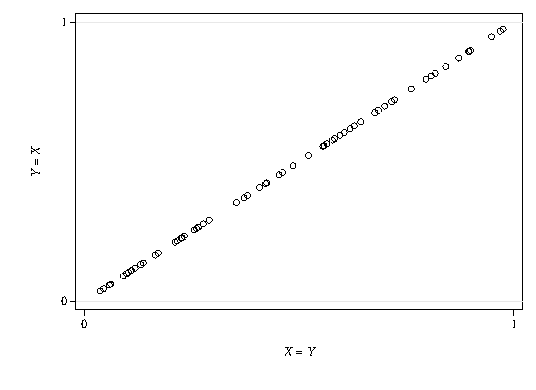
\includegraphics[width=.32\textwidth]{images/correlate_pos.pdf}
  	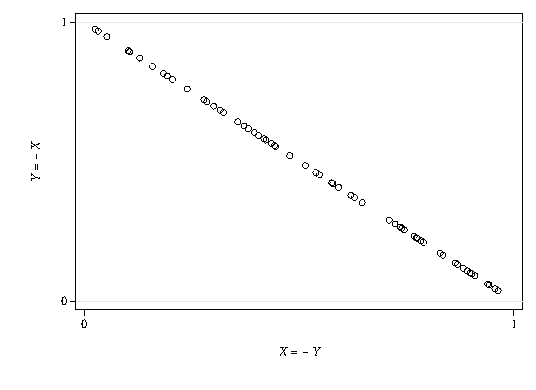
\includegraphics[width=.32\textwidth]{images/correlate_neg.pdf}
  	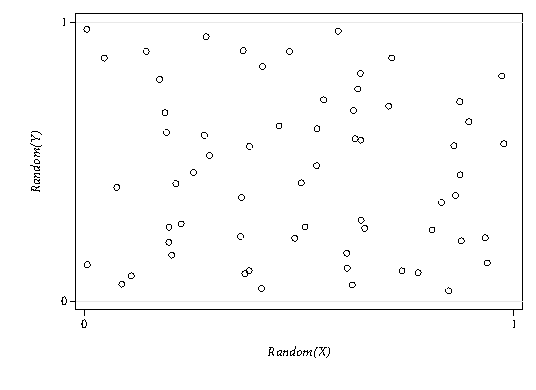
\includegraphics[width=.32\textwidth]{images/correlate_rnd.pdf}

  	\caption[`Extreme' correlation coefficients]{\label{fig:correlation_examples}%
  	`Extreme' correlation coefficients: from left to right, %
    $\rho = +1$, $\rho = -1$ and $\rho \approx 0$. %
    Simulated from random data.}
  \end{figure}%

  The formula that is generally used for measuring correlation is Pearson's $\rho$, a coefficient measure that divides the \emph{covariance} of $X$ and $Y$ by the product of their standard deviations $\sigma_X$ and $\sigma_Y$, which are themselves the square roots of the variance in $X$ and $Y$:

  $$\text{Cov}[X,Y] = \frac{\sum{(X_i-\bar X_i)(Y_i-\bar Y_i)}}{N} \quad \text{and} \quad \rho_{X,Y} = \text{corr}[X] = \frac{\text{Cov}[X,Y]}{\sigma_X \sigma_Y} = \frac{\text{Cov}[X,Y]}{\sqrt{\text{Var}[X] \text{Var}[Y]}}$$

  Pearson's $\rho$ is calculated out of the sample estimates that we hold for the means $\bar X$ and $\bar Y$, which we write $\mu_X$ and $\mu_Y$ at the level of the population, or universe, from which we have sampled our data. Identically, Pearson's $\rho$ depends on the standard deviation of each variable in the sample, which we denote as $s_X$ and $s_Y$ for their sample values. Since it relies on estimated parameters, the correlation coefficient can be tested for statistical significance, in order to verify that it is different from $(H_0): \rho = 0$ at a given level of confidence.

  Stata offers two different commands for correlation with Pearson's $\rho$, both very straightforward. 

\subsection{Exporting correlation matrixes}%
  \index{Correlation!Matrixes}%
  \index{Correlation!Exporting results}

When you are done with visual inspection with scatterplots (\texttt{sc}), compute correlation coefficients for your selection of variables with the \cmd{pwcorr} command. The \texttt{pw} prefix in the name of the command stands for \emph{pairwise} case deletion of missing data: it means that this command will calculate each correlation coefficient on the specific sample of observations for which the pair of variables is not missing.

\label{casewise}Pairwise case deletion can create serious validity issues if you need to compare coefficients over variables with different patterns of missing data, for which \emph{listwise} case deletion with the \cmd{corr}{correlate} command is more reliable. This situation is probably not so frequent with social science data. Note that, despite their names, pairwise and listwise case deletion are non-destructive subsetting operations that leave the data intact. More information is available at \statacode{help corr} from within Stata or \href{http://www.stata.com/help.cgi?correlate}{from its website}.

There are a few options to export your correlation matrixes from Stata to a spreadsheet editor or to a text document. The safest solution is always to generate a separate file that can be saved and archived for reference, rather than copying and pasting. This applies to both correlation and scatterplot matrixes.

Table~\ref{tbl:correlate_export} shows two options. The most straightforward command to export a correlation matrix is \cmd{mkcorr}, which can export to comma-separated format (\ext{.csv}) in one line. The recommended alternative is to use the more polyvalent \cmd{estout} package, which produces very clean results. The documentation page for \cmd{estout} has plenty more options and its \href{http://repec.org/bocode/e/estout/estpost.html#estpost112}{online documentation} is very handy too.

\begin{table}[htp]
	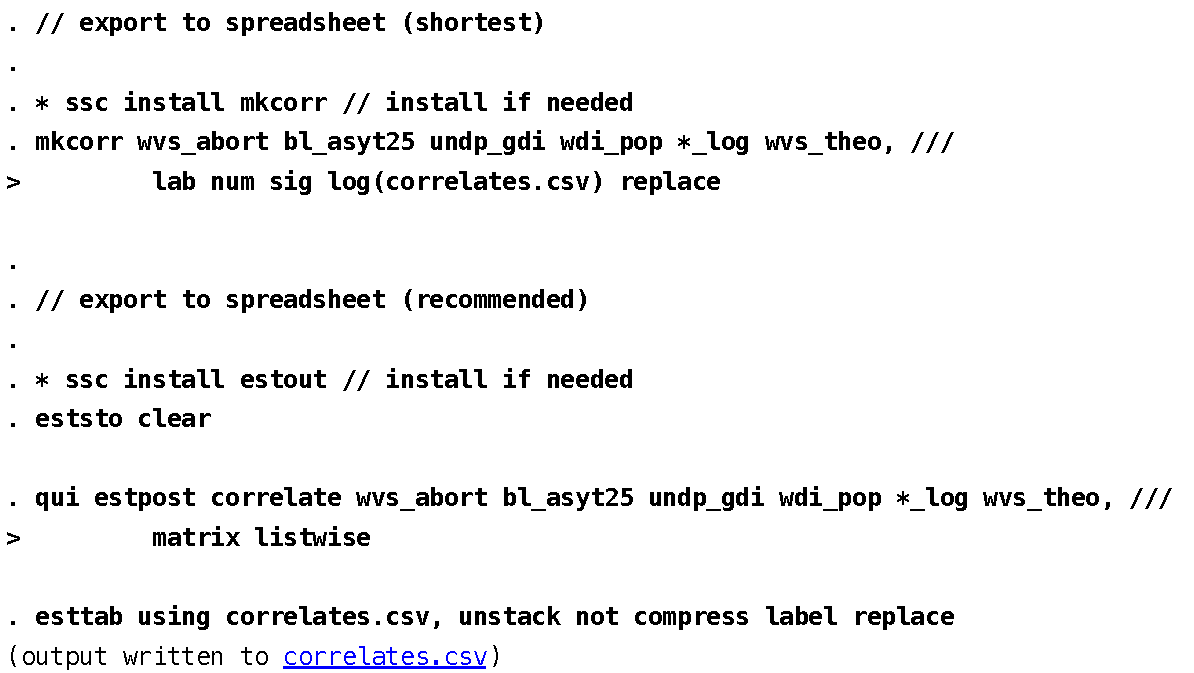
\includegraphics[scale=.5]{images/correlate_export.pdf}

	\caption[Exporting a correlation matrix with \cmd{mkcorr} and \cmd{estout}]{\label{tbl:correlate_export}%
	Exporting a correlation matrix with \cmd{mkcorr} and \cmd{estout}. %
  See \statacode{help estout} and related online documentation for options. %
	\qog}
\end{table}%

Table~\ref{tbl:pwcorr} shows Stata output for the \cmd{pwcorr} command with the \opt{obs}{pwcorr} and \opt{star(.05)}{pwcorr} options, which respectively add the number of pairwise observations and appose an asterisk next to statistically significant correlations at $p < .05$.\footnote{Remember not to vow any cult to the statistical significance asterisk. The magnitude of the correlation coefficient, \ie its closeness to $-1$ or $+1$, is a more reliable metric (and both quickly corroborate). Visual inspection certainly trumps both measures if your goal is to detect genuinely linear relationships.} This type of table is called a \emph{correlation matrix} and is frequently produced prior to linear regression models.

\begin{table}[htp]
	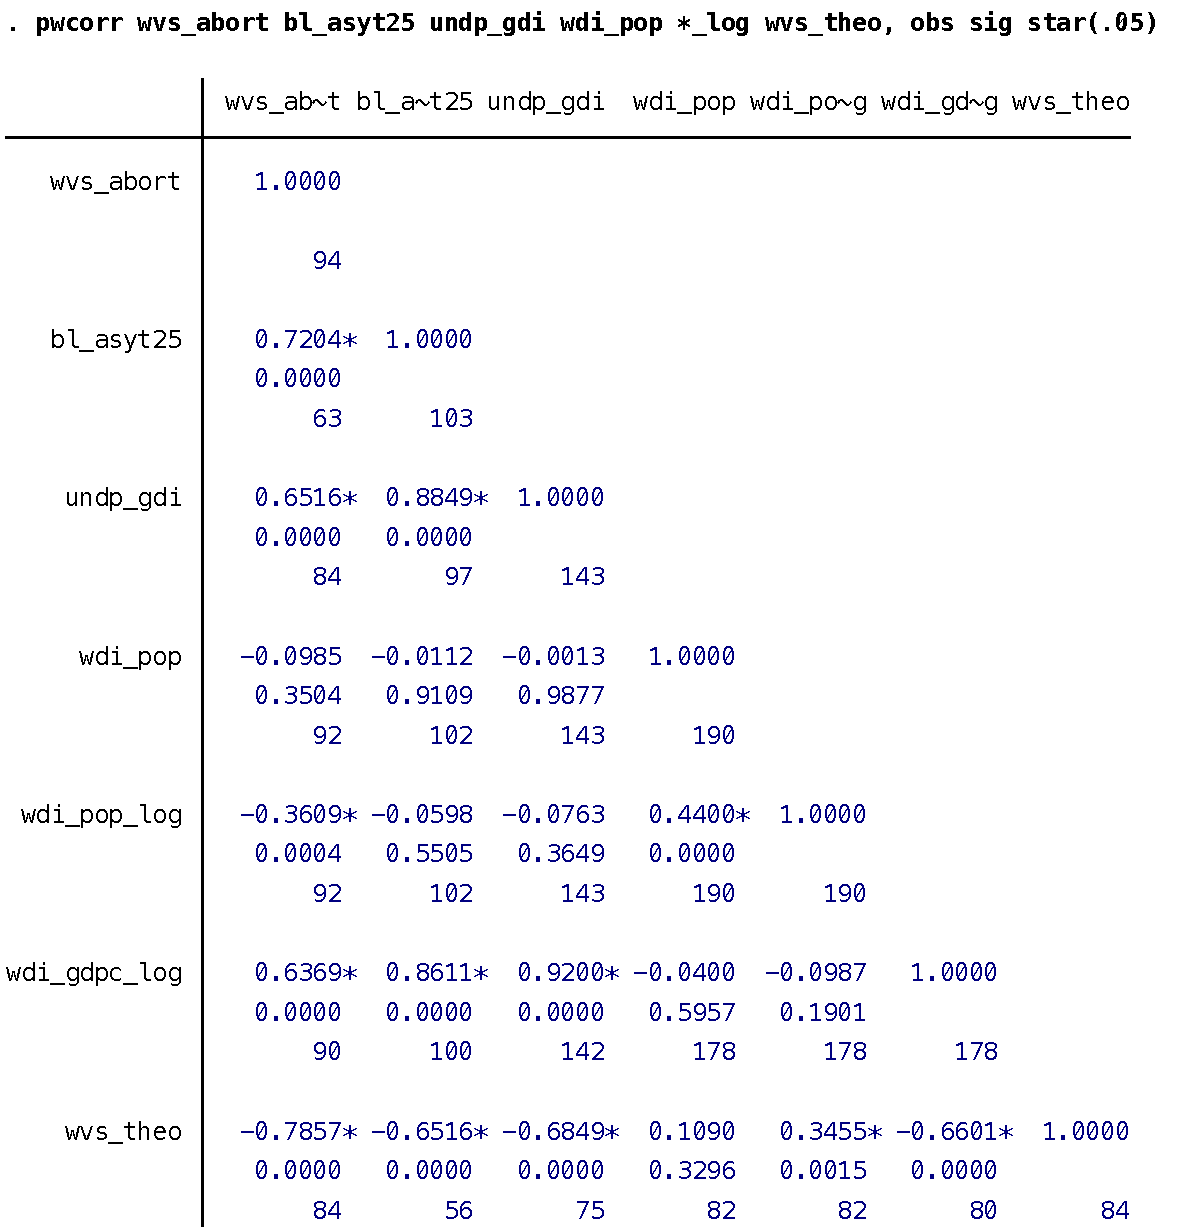
\includegraphics[scale=.5]{images/abortion_pwcorr.pdf}

	\caption[Correlation matrix with \cmd{pwcorr}]{\label{tbl:pwcorr}%
	Correlation matrix produced with \texttt{pwcorr, obs star(.05)}. %
  \qog}
\end{table}%

We passed the previously introduced \texttt{wvs\_abort} (support for abortion) and \texttt{bl\_asyt25} (mass education) variables to the correlation matrix, as well as a few other variables:

\begin{enumerate}
	\item[\emph{Gender equality}] We first added \texttt{undp\_gdi}, a measure of gender equality from the United Nations Development Programme (briefly mentioned in a footnote at p.~\pageref{fn:gdi_gem});

	\item[\emph{Wealth}] We then added recent estimates for GDP/capita by the World Bank as part of its World Development Indicators (\texttt{wdi\_gdpc});

	\item[\emph{Theocracy}] We then chose to add \texttt{wvs\_theo}, a \WVS{} variable that measures support in theocracy, which we expect to vary in a diametrically opposed direction to support for abortion in the data.\footnote{The measure comes on a grossly normal 0--1 scale and aggregate four other survey questions from the \WVS{}. The reliability of the coding and scaling could require additional checks on the initial measures.}

	\item[\emph{Population}] Finally, we added \texttt{wdi\_pop}, a measure of population, in its normal metric (number of de facto residents) and in its logarithmic transformation, as population follows a highly skewed distribution with tons of micro-states versus a handful of growing giant countries.
\end{enumerate}

In our matrix, the correlation coefficients for the abortion, education, gender and wealth measures are all positive and statistically significant. Most importantly, their strength is probably twice the strength of what would be a reasonably strong correlation in social science data. This pattern has several implications for our subsequent analysis:

\begin{enumerate}
	\item At the empirical level, these variables identify clusters of observations in the data. Typically, in comparison to the rest of the sample, \textsc{weird} countries\footnote{The \textsc{weird}s designate Western, Educated, Industrialized, Rich and Democratic countries, in which individuals think and behave differently than in other parts of the world. This has implications especially for experimental research that overwhelmingly relies on Western subjects. The argument is developed in \cite{HenrichHeine:2010a}.} all have high levels of support for abortion, educational attainment, economic wealth and gender equality. The rest of the distribution might contain other clusters, for which you should at least provide a tentative description. The existing literature can also help you detect other characteristics of these clusters that your variables might not have fully captured.

	\item At the statistical level, the clusters of observations characterized by either high or low levels of education, wealth and gender equality are going to account for a substantial fraction of the covariance. Their distribution around the mean, as shown in Figure~\ref{fig:correlation_variance}, can later affect our estimates of the model parameters. You will therefore want to check for outliers that might distort, exaggerate or downplay the correlational pattern.
\end{enumerate}

The correlation coefficients for support in theocracy (\texttt{wvs\_theo}) differ in several respects. First of all, they are computed on slightly smaller samples due to missing data. Most importantly, the coefficients show that support for theocracy is negatively correlated with the other variables examined, somewhere in the same (relatively high) order of magnitude observed in other variables, and somewhere in the same satisfactory levels of statistical significance.

Last, the correlation coefficients for \texttt{wdi\_pop} and its natural logarithm show the corrective effects of variable transformation on the estimation of significance levels. If you re-run the \cmd{pwcorr} command shown in Table~\ref{tbl:pwcorr} with the \opt{sig}{pwcorr} option, Stata will show you the $p$-value for each correlation coefficient. This will show clear improvements in coefficient strength and statistical significance for the more normally distributed \texttt{wdi\_pop\_log} variable.

  \index{Spearman's $\rho$|see{correlation}}\index{Kendall's $\tau$|see{correlation}}%
  \paragraph{Additional options for ordinal data} If your data use a low number of dimensions, additional measures of correlation might come in handy.

  Pearson's $\rho$ is very effective at detecting correlation with continuous data where correlation depends on the values of the observations. However, if the correlational pattern derives from the ranks of the observations, as with $k$-point scales, Spearman's $\rho$ (\cmd{spearman}) can be more effective at detecting the relationship, because it looks for monotonicity instead of linearity.\footnote{Monotonicity disregards the actual numeric values of the data and focuses on the order of the values. For example, if you are looking at a variable scaled from \texttt{1 "Strongly agree"} to \texttt{5 "Strongly disagree"}, or from \texttt{0 "Never contracted"} to \texttt{3 "Full-time contract"}, the order of the categories takes over the values in meaningfulness.} The command works pretty much like \cmd{corr}.

  Furthermore, if your dataset relies on a relatively small number of observations, you should also give a try to Kendall's $\tau$ (\cmd{ktau}), which takes some time to compute. If you are hesitant about the relevance of the scaling used in some variables, running through all commands will generally help understand their correlational pattern, and will also prevent your analysis from methodological straitjacketing.

  Even when the relationship \emph{is} linear and measured as such, you still need to compare your measures of correlation with your theoretical expectations. A correlation coefficient of $\rho = 0.6$ can be empirically insufficient if your model predicted a stronger linear association between the two variables.

The examples below use variables from the \qog{} dataset:%

\begin{docspec}
  * example data\\%
  use bl\_lu\_25mf undp\_gii wvs\_abort wvs\_theo unna\_pop wdi\_gdpc using data/qog2013, clear\\%
  * log-transformations\\%
  gen log\_pop = ln(unna\_pop)\\%
  la var log\_pop "Log(Population)"\\%
  gen log\_gdpc = ln(wdi\_gdpc)\\%
  la var log\_gdpc "Log(GDP per capita)"
\end{docspec}

%
\paragraph{Formatting}%
  \index{Correlation!Matrixes}%
  %
  Table~\ref{tbl:estout_corr} shows a correlation matrix exported with the \cmd{estout} package, as shown at p.~\pageref{tbl:correlate_export}.%

  %
  % The numbering system saves space on paper, and columns are aligned on the decimal point to increase readability. Variable labels are preferable to less informative variable names. Last, remember to stick a complete caption. \emph{Note:} if you want to use cell colors to `warm up' the table, please feel free to do so, using a soft color theme.
  %
\begin{fullwidth}
	\begin{table}
		\footnotesize
    %
    {
\def\sym#1{\ifmmode^{#1}\else\(^{#1}\)\fi}
\begin{tabular}{l*{8}{c}}
\hline\hline
                &\multicolumn{8}{c}{}                                                                                                                                   \\
                &(1)&(2)&(3)&(4)&(5)&(6)&(7)&(8) \\
\hline
(1) No Schooling, Female and Male (25+)&        1         &                  &                  &                  &                  &                  &                  &                  \\
(2) Gender Inequality Index&    0.744\sym{***}&        1         &                  &                  &                  &                  &                  &                  \\
(3) Population      &    0.221         &    0.269         &        1         &                  &                  &                  &                  &                  \\
(4) GDP per Capita, PPP (Constant International USD)&   -0.606\sym{***}&   -0.828\sym{***}&   -0.121         &        1         &                  &                  &                  &                  \\
(5) Abortion is justifiable&   -0.517\sym{***}&   -0.729\sym{***}&  -0.0934         &    0.750\sym{***}&        1         &                  &                  &                  \\
(6) Support for theocracy&    0.579\sym{***}&    0.834\sym{***}&   0.0952         &   -0.763\sym{***}&   -0.865\sym{***}&        1         &                  &                  \\
(7) Log(Population) &    0.125         &    0.255         &    0.621\sym{***}&   -0.140         &   -0.274         &    0.219         &        1         &                  \\
(8) Log(GDP per capita)&   -0.762\sym{***}&   -0.835\sym{***}&   -0.143         &    0.903\sym{***}&    0.648\sym{***}&   -0.700\sym{***}&   -0.106         &        1         \\
\hline
Observations    &       41         &                  &                  &                  &                  &                  &                  &                  \\
\hline\hline
\multicolumn{9}{l}{\footnotesize \sym{*} \(p<0.05\), \sym{**} \(p<0.01\), \sym{***} \(p<0.001\)}\\
\end{tabular}
}

		%
		\caption{Correlation output produced with \cmd{estout} and edited by adding variable numbers.}
		\label{tbl:estout_corr}
	\end{table}
\end{fullwidth}

\begin{docspec}
  * export correlation matrix with -estout-\\
  keep wvs\_abort bl\_lu\_25mf log\_*\\
  qui estpost correlate *, matrix listwise\\
  esttab using correlates.csv, ///\\%
    replace unstack not compress label nonum
\end{docspec}

  % \begin{frame}{Exercise}
  % 
  %     \begin{exampleblock}{Ex~7.1. Quality of Government 2011}
  % 
  %       \begin{itemize}
  %         \item Variables: \texttt{d wdi\_brd wdi\_mege wdi\_pb2 wdi\_the}
  %         \item Inspect and plot the correlation matrix.
  %       \end{itemize}
  % 
  %     \end{exampleblock}
  % 
  % 
  %   \begin{exampleblock}{Ex~7.2. Quality of Government 2011}
  %       
  %       \begin{itemize}
  %         \item Variables: \texttt{d wdi\_puhegdp wdi\_the wdi\_prhe}
  %         \item Visualize and export the correlations and scatterplots.
  %       \end{itemize}
  %       
  %   \end{exampleblock}
  % 
  % 
  % \end{frame}
